\section{Ergebnisse}
\label{sec:ergebnisse}
\subsection{Versuchteil 1:}
 
 \begin{itemize}
 	\item Interpretation mit Reaktionsgleichung Sauerstoff\\
 		\begin{flalign}
 			\ce{O2 + 2 e^- + 2 H2O -> H2O2 + 2 OH-}
 		\end{flalign}
 		\begin{flalign}
 		\ce{H2O2 + 2 e^- -> 2 OH^-}
 		\end{flalign}
 	\item Vergleich Polarogramm geglättet und ungeglättet
 	\item Zuordnung Begründen
 \end{itemize}
 
 %Start
 \begin{figure}[h!]
 	\centering
 	\includegraphics[width=0.9\textwidth]{img/Daten_farbig2}
 	\caption{Strom-Spannungskurven (Polarogramme) des Versuchsteils 1}
 	\label{fig:daten_farbig}
 \end{figure}
 \FloatBarrier
 %Ende     
 %Tabelle START
 \vspace*{-2.5mm}
 \renewcommand{\arraystretch}{1.2}
 \begin{table}[h!]
 	\centering
 	\caption{Zuordnung der Peaks den Elementen des Multielementencocktails}
 	\label{tab:peaks}
 	%\resizebox{10cm}{!}{
 	\begin{tabulary}{\textwidth}{C|CCCC}
 		\hline
 		\textbf{Element} &  \textbf{Kupfer-\ce{Cu}}  &\textbf{Blei-\ce{Pb}}& \textbf{Cadmium-\ce{Cd}} & \textbf{Zink-\ce{Zn}}\\ 
 		\hline
 		\textbf{Peak} &1&2&3&4\\
 		\hline
 	\end{tabulary}
 	%}
 \end{table}
 \FloatBarrier
 \vspace*{-2.5mm}
 %Tabelle ENDE
 
 
\newpage
 
 \subsection{Versuchsteil 2:}

\begin{itemize}
	\item  Polarogramm Probe mit Aufstockungen ?
	\item  Quantitative Auswertung des Programms
	\item  MANUELLE KALIBRIERGERADE !!
	\item  Aliquotierfaktor\\
\end{itemize}

\textbf{Berechnung der Blei-Standard-Zugaben-Konzentration:}
\begin{flalign}
	V_{\text{Standard-Zugabe}} * c_{\text{Standard-Zugabe}} &= V_{\text{Lösung}} * c_{\text{Lösung}}\\
	c_{\text{Lösung}} 	&= \frac{V_{\text{Standard-Zugabe}} }{V_{\text{Lösung}}} * c_{\text{Standard-Zugabe}}		
\end{flalign}
\begin{flalign}
	c_{\text{Lösung},1} &=\frac{\SI{200e-6}{\liter}}{\SI{25e-3}{\liter}} * \SI{1000}{\milli \gram \per \liter}\\
	&= \underline{\SI{8}{\milli \gram \per \liter}	}\\[3mm]
	c_{\text{Lösung},2} &=\frac{\SI{400e-6}{\liter}}{\SI{25e-3}{\liter}} * \SI{1000}{\milli \gram \per \liter}\\
	&= \underline{\SI{16}{\milli \gram \per \liter}	}
\end{flalign}

 %Tabelle START
\vspace*{-2.5mm}
\renewcommand{\arraystretch}{1.2}
\begin{table}[h!]
	\centering
	\caption{Messreihe 1 mit berechneten Leistungen}
	\label{tab:messreihe1}
	%\resizebox{10cm}{!}{
	\begin{tabulary}{\textwidth}{C|CCC}
		\hline
		\textbf{Konzentration der Bleizugabe in \si{\milli \gram \per \liter}} &  \textbf{Spannung in \si{\volt}}  &\textbf{Stromstärke in \si{\nano \ampere}}& \textbf{Leistung in \si{\nano \watt}}\\ 
		\hline
		0 	&-0,376	&-113,0	&42,488\\
		0 	&-0,376	&-112,5	&42,300\\
		8 	&-0,376	&-268,2	&100,843\\
		8 	&-0,376	&-266,6	&100,242\\
		16 	&-0,376	&-422,8	&158,973\\
		16 	&-0,382	&-416,0	&158,912\\
		\hline
	\end{tabulary}
	%}
\end{table}
\FloatBarrier
\vspace*{-2.5mm}
%Tabelle ENDE
 %Tabelle START
\vspace*{-2.5mm}
\renewcommand{\arraystretch}{1.2}
\begin{table}[h!]
	\centering
	\caption{Messreihe 2 mit berechneten Leistungen}
	\label{tab:messreihe2}
	%\resizebox{10cm}{!}{
	\begin{tabulary}{\textwidth}{C|CCC}
		\hline
		\textbf{Konzentration der Bleizugabe in \si{\milli \gram \per \liter}} &  \textbf{Spannung in \si{\volt}}  &\textbf{Stromstärke in \si{\nano \ampere}}& \textbf{Leistung in \si{\nano \watt}}\\ 
		\hline
		0 	&-0,382	&-129,3	&49,393\\
		0 	&-0,382	&-139,2	&53,174\\
		8 	&-0,382	&-286,2	&109,328\\
		8 	&-0,382	&-282,2	&107,800\\
		16 	&-0,382	&-425,1	&162,388\\
		16 	&-0,382	&-424,0	&161,968\\
		\hline
	\end{tabulary}
	%}
\end{table}
\FloatBarrier
\vspace*{-2.5mm}
%Tabelle ENDE

%\begin{figure}[h!]
%	\begin{center}
%		\resizebox{0.95\textwidth}{!}{
%		\begin{tikzpicture}[trim axis left, trim axis right]
%		\begin{axis}[
%		axis lines = middle,
%		width = 20cm,
%		height = 10cm,
%		xmin = -10,
%		xmax = 20,
%	%	ymin = -0.1,
%	%	ymax = 0,
%	%	ytick = {-4.5,-4,...,-1},
%	%	xtick = {-10,-9,...,20},
%		ylabel={Leistung in \si{\nano \watt}},
%		y label style={at={(0.25,0.40)}, rotate=90},
%		xlabel={Konzentration der Blei-Standard-Zugabe in \si{\milli \gram \per \milli \liter}},
%		legend style={at={(0.75,0.45)},anchor=west}
%		]
%		\addplot table {datenm1.dat};
%		\addplot +[mark=none, dashed, black, domain=-10:20] {-2e-8*x-1e-7};
%		\addplot table {datenm2.dat};
%		\addplot +[mark=none, dotted, black, domain=-10:20] {-2e-5*x - 0.0001};
%		
%		\legend{Messreihe 1, Regression Messreihe 1,Messreihe 2, Regression Messreihe 2};
%		\end{axis}
%		\end{tikzpicture}
%			}
%		\caption{Berechnete Leitungen in Abhängigkeit von der Konzentration der Blei-Standardzugabe (siehe Tab. \ref{tab:messreihe1} und Tab. \ref{tab:messreihe2})}
%		\label{dia:lnr/lnc}
%	\end{center}
%\end{figure}
%\FloatBarrier
%\vspace*{-5mm}

\pagebreak

 \includepdf[pages=2-5]{Daten_farbig2}